%% 03.tex
\documentclass[platex,dvipdfmx]{jsreport}

\usepackage{graphicx}
\graphicspath{{./images/}{../images/}}
\usepackage{pdfpages}
\usepackage{tikz}
\usepackage{xcolor}
\definecolor{UD_GREEN}{HTML}{03af7a}
\usepackage{bm}
\usepackage[left=30truemm]{geometry}
\usepackage{amsmath,amssymb}
\numberwithin{equation}{section}



\begin{document}

\chapter{本論}

\section{手法}
\subsection{逆オパール構造}
逆オパール構造の球の半径$r / a$を徐々に変化させていった際のバンドギャップの変化を観察した。このときのバンドギャップの変化を$\epsilon = 5, 10, 13, 15$のそれぞれについて行い、各$\epsilon$におけるバンドギャップの数とギャップ-ミッドギャップ比の変化を観察し最適な構造を検討した。
% \subsection{ウッドパイル構造}
% ウッドパイル構造の誘電体棒の幅$w / a$を徐々に変化させていった際のバンドギャップの変化を観察した。このときのバンドギャップの変化を$\epsilon = 5, 10, 13, 15$のそれぞれについて行い、各$\epsilon$におけるバンドギャップの数とギャップ-ミッドギャップ比の変化を観察し最適な構造を検討した。
% \subsection{ヤブロノバイト構造}
% ヤブロノバイト構造の誘電体円柱の半径$r / a$を徐々に変化させていった際のバンドギャップの変化を観察した。このときのバンドギャップの変化を$\epsilon = 5, 10, 13, 15$のそれぞれについて行い、各$\epsilon$におけるバンドギャップの数とギャップ-ミッドギャップ比の変化を観察し最適な構造を検討した。
% \subsection{2次元構造の積み重ね}
% 2次元結晶の積み重ねにより作成された3次元構造の空気柱の半径$r / a$を徐々に変化させていった際のバンドギャップの変化を観察した。このときのバンドギャップの変化を$\epsilon = 5, 10, 12, 15$のそれぞれについて行い、各$\epsilon$におけるバンドギャップの数とギャップ-ミッドギャップ比の変化を観察し最適な構造を検討した。


\section{結果}
\subsection{逆オパール構造}
逆オパール構造に配置されている球の半径$r / a$を0.01ずつ変化させ、ギャップ-ミッドギャップ比の変化を観察した。この変化を$\epsilon = 5, 10, 13, 15$のそれぞれについて行った。

このときの各$\epsilon$におけるギャップマップを以下の図\ref{fig:gapmap_inv_opal_e-5}から図\ref{fig:gapmap_inv_opal_e-15}に示す。

\begin{figure}[h]
  \begin{minipage}[h]{0.5\linewidth}
    \centering
    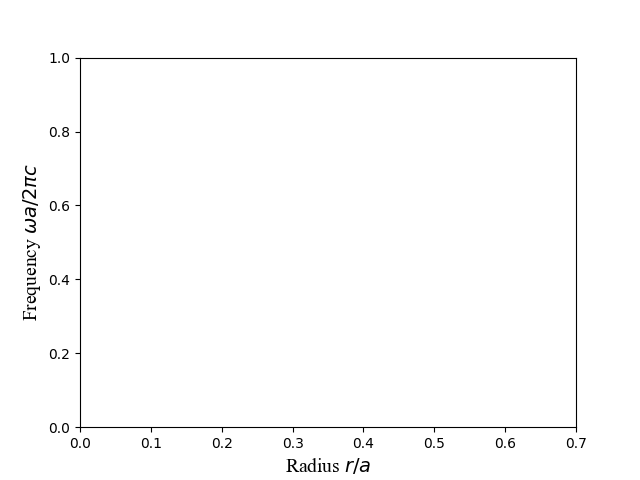
\includegraphics[keepaspectratio, scale=0.45]{results/gap_map/inv_e-5.png}
    \caption{逆オパール構造のギャップマップ($\epsilon = 5$)}
    \label{fig:gapmap_inv_opal_e-5}
  \end{minipage}
  \begin{minipage}[h]{0.5\linewidth}
    \centering
    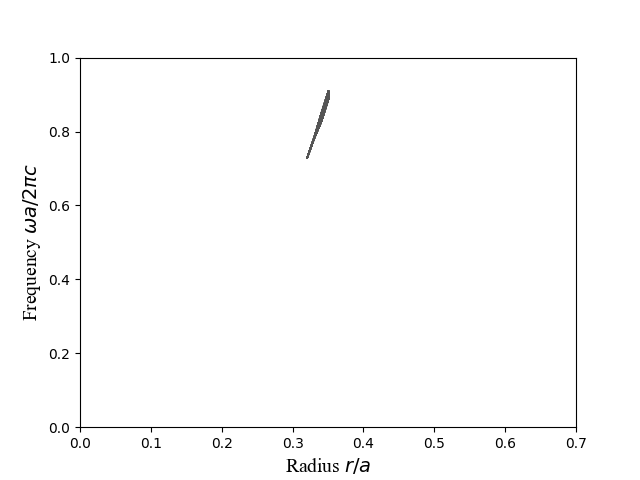
\includegraphics[keepaspectratio, scale=0.45]{results/gap_map/inv_e-10.png}
    \caption{逆オパール構造のギャップマップ($\epsilon = 10$)}
    \label{fig:gapmap_inv_opal_e-10}
  \end{minipage}
\end{figure}

\begin{figure}[h]

  \begin{minipage}[h]{0.5\linewidth}
    \centering
    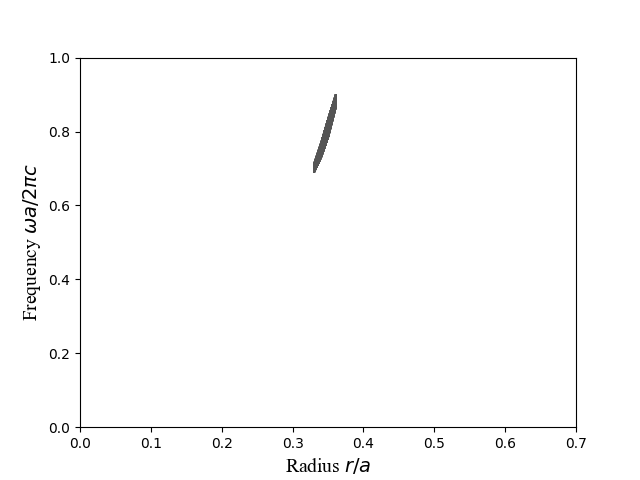
\includegraphics[keepaspectratio, scale=0.45]{results/gap_map/inv_e-13.png}
    \caption{逆オパール構造のギャップマップ($\epsilon = 13$)}
    \label{fig:gapmap_inv_opal_e-13}
  \end{minipage}
  \begin{minipage}[h]{0.5\linewidth}
    \centering
    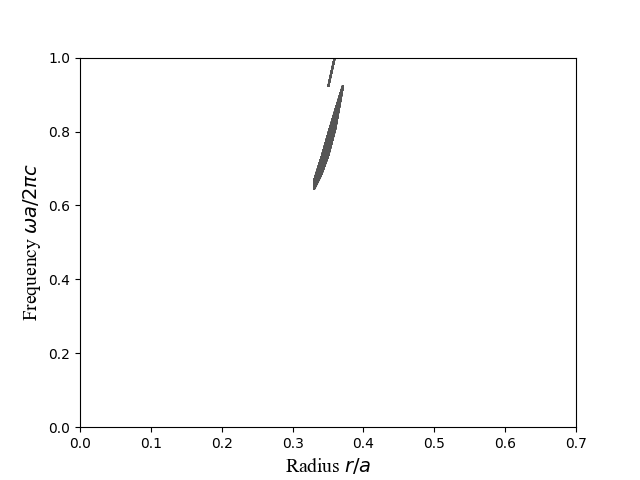
\includegraphics[keepaspectratio, scale=0.45]{results/gap_map/inv_e-15.png}
    \caption{逆オパール構造のギャップマップ($\epsilon = 15$)}
    \label{fig:gapmap_inv_opal_e-15}
  \end{minipage}
\end{figure}

$\epsilon = 5$のとき、バンドギャップは生じなかった。一方で$\epsilon = 10, 13, 15$のときはバンドギャップが生じた。$\epsilon = 10, 13$のときはバンドギャップは1つであったが、$\epsilon = 15$のときはバンドギャップは2つであった。

ギャップマップの形状はいずれも似通っており、半径$r / a$が大きくなるほど周波数$\omega a / 2 \pi c$が大きくなっていることが確認できた。

次に、各$\epsilon$において球の半径とギャップ-ミッドギャップ比の関係を図\ref{fig:inv_opal}に示す。

  
\begin{figure}[htbp]
  \centering
  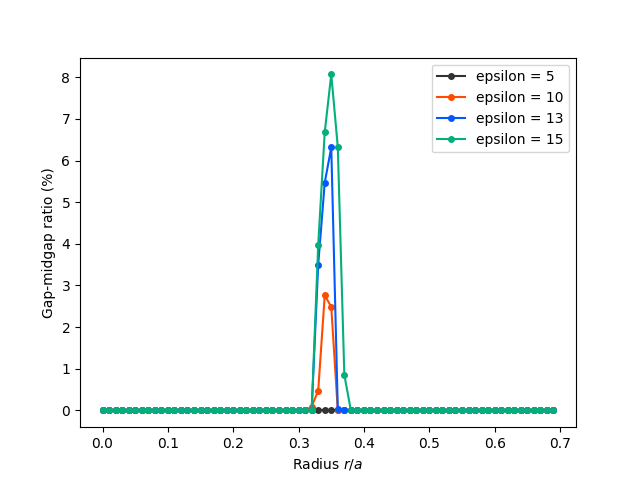
\includegraphics[width=0.8\linewidth]{results/gap_midgap_ratio/inv_opals.png}
  \caption{逆オパール構造の球の半径$r / a$を変化させた際のギャップ-ミッドギャップ比の変化}
  \label{fig:inv_opal}
\end{figure}

$\epsilon = 5$のときはバンドギャップは確認できなかった。
$\epsilon = 10, 13, 15$のいずれもバンドギャップは確認できそのグラフの形状はいずれも狭い$r / a$の範囲の中で急激に変化していることが確認できる。
\\
$\epsilon = 10$のとき、$0.33 \leq r / a \leq 0.36$の間でギャップが発生し、$r / a = 0.35$でギャップ-ミッドギャップ比は最大となりその値は$2.764 \%$だった。
\\
$\epsilon = 13$のとき、$0.34 \leq r / a \leq 0.37$の間でギャップが発生し、$r / a = 0.36$でギャップ-ミッドギャップ比は最大となりその値は$6.317 \%$だった。
\\
$\epsilon = 15$のとき、$0.34 \leq r / a \leq 0.38$の間でギャップが発生し、$r / a = 0.36$でギャップ-ミッドギャップ比は最大となりその値は$8.069 \%$だった。

更に詳細にギャップ-ミッドギャップ比が最大となる$r / a$の値を求めるために、$0.34 \leq r / a \leq 0.37$の範囲で$r / a$を0.0001ずつ変化させた際のギャップ-ミッドギャップ比の変化を図\ref{fig:inv_opal_detail}に示す。

% \clearpage

% \subsection{ウッドパイル構造}
% ウッドパイル構造中に配置されている誘電体棒の半径$w / a$を0.01ずつ変化させ、ギャップ-ミッドギャップ比の変化を観察した。この変化を$\epsilon = 5, 10, 13, 15$のそれぞれについて行った。

% このときの各$\epsilon$におけるギャップマップを以下の図\ref{fig:gapmap_woodpile_e-5}から図\ref{fig:gapmap_woodpile_e-15}に示す。
% \begin{figure}[h]
%   \begin{minipage}[h]{0.5\linewidth}
%     \centering
%     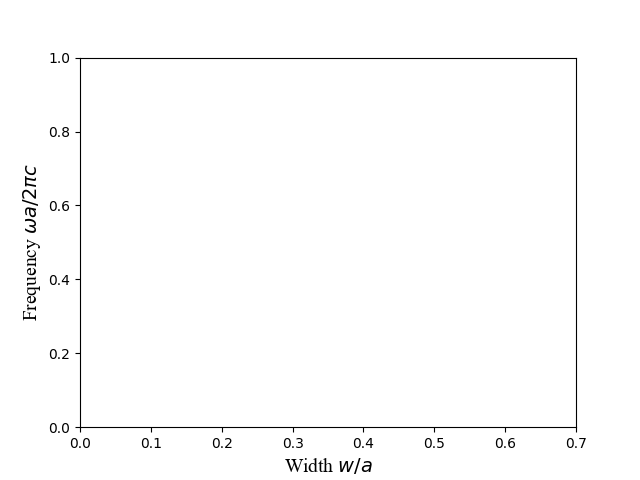
\includegraphics[keepaspectratio, scale=0.45]{results/gap_map/woodpile-2_e-5.png}
%     \caption{ウッドパイル構造のギャップマップ($\epsilon = 5$)}
%     \label{fig:gapmap_woodpile_e-5}
%   \end{minipage}
%   \begin{minipage}[h]{0.5\linewidth}
%     \centering
%     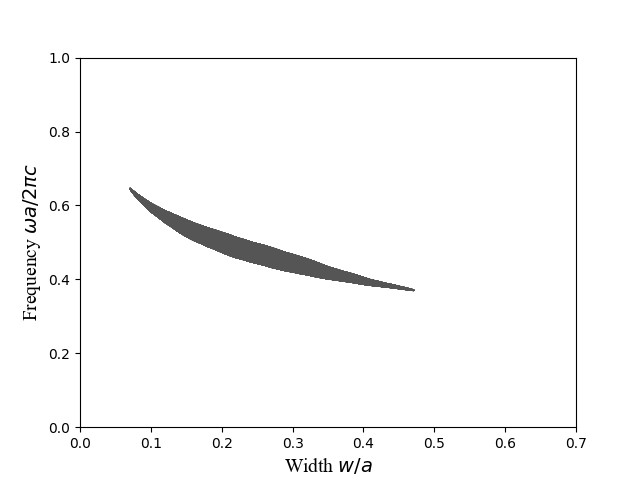
\includegraphics[keepaspectratio, scale=0.45]{results/gap_map/woodpile-2_e-10.png}
%     \caption{ウッドパイル構造のギャップマップ($\epsilon = 10$)}
%     \label{fig:gapmap_woodpile_e-10}
%   \end{minipage}
% \end{figure}
% \begin{figure}[h]
%   \begin{minipage}[h]{0.5\linewidth}
%     \centering
%     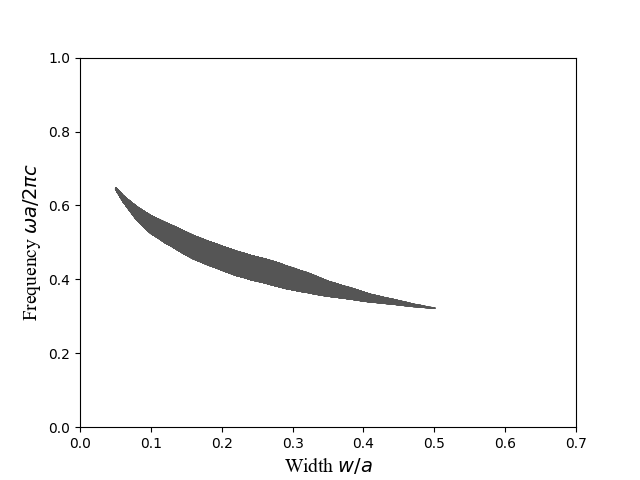
\includegraphics[keepaspectratio, scale=0.45]{results/gap_map/woodpile-2_e-13.png}
%     \caption{ウッドパイル構造のギャップマップ($\epsilon = 13$)}
%     \label{fig:gapmap_woodpile_e-13}
%   \end{minipage}
%   \begin{minipage}[h]{0.5\linewidth}
%     \centering
%     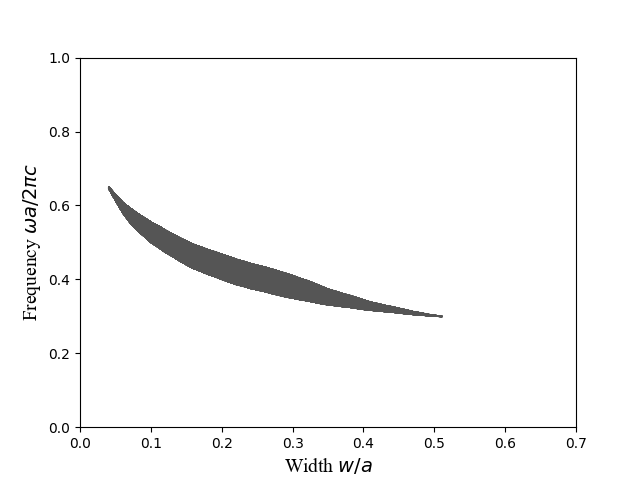
\includegraphics[keepaspectratio, scale=0.45]{results/gap_map/woodpile-2_e-15.png}
%     \caption{ウッドパイル構造のギャップマップ($\epsilon = 15$)}
%     \label{fig:gapmap_woodpile_e-15}
%   \end{minipage}
% \end{figure}

% $\epsilon = 5$のときはバンドギャップの発生は確認できなかった。一方で$\epsilon = 10, 13, 15$のときはバンドギャップが生じた。バンドが生じた場合、ギャップマップの形状は非常に似通っていた。

% 次に各$\epsilon$におけるギャップ-ミッドギャップ比を誘電体棒幅$w / a$を横軸にとってプロットしたグラフを図\ref{fig:woodpile}に示す。 



% \begin{figure}[htbp]
%   \centering
%   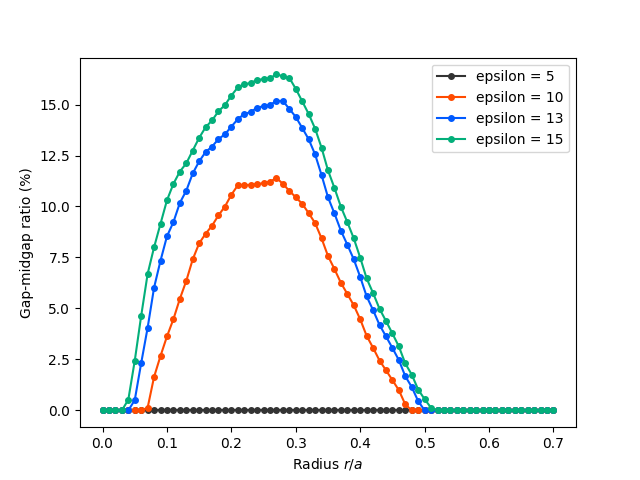
\includegraphics[width=0.8\linewidth]{results/gap_midgap_ratio/woodpile-2.png}
%   \caption{ウッドパイル構造の誘電体棒の幅$w / a$を変化させた際のギャップ-ミッドギャップ比の変化}
%   \label{fig:woodpile}
% \end{figure}

% $\epsilon = 10$のとき、$0.08 \leq w / a \leq 0.48$の範囲でギャップが生じ、$ w / a = 0.28$でギャップ-ミッドギャップ比は最大となりその値は$11.394 \%$だった。\\
% $\epsilon = 13$のとき、$0.06 \leq w / a \leq 0.51$の範囲でギャップが生じ、$w / a = 0.29$のときにギャップ-ミッドギャップ比は最大となりその値は$15.176 \%$だった。\\
% $\epsilon = 15$のとき、$0.05 \leq w / a \leq 0.52$の範囲でギャップが生じ、$w / a = 0.28$のときにギャップ-ミッドギャップ比は最大となりその値は$16.478 \%$だった。
% バンドギャップの生じる領域幅も、ギャップ-ミッドギャップ比が最大となる幅もほとんど同じであることが確認できた。

% \clearpage
% \subsection{ヤブロノバイト構造}
% ヤブロノバイト構造中に配置されている空気円柱の半径$r / a$を0.01ずつ変化させ、ギャップ-ミッドギャップ比の変化を観察した。この変化を$\epsilon = 5, 10, 13, 15$のそれぞれについて行った。

% 各$\epsilon$におけるギャップマップを以下の図\ref{fig:gapmap_yablonovite_e-5}から図\ref{fig:gapmap_yablonovite_e-15}に示す。

% \begin{figure}[h]
%   \begin{minipage}[h]{0.5\linewidth}
%     \centering
%     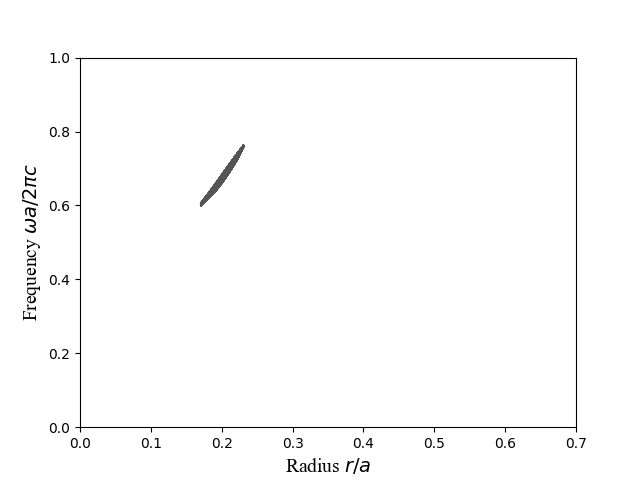
\includegraphics[keepaspectratio, scale=0.45]{results/gap_map/yablonovite_e-5.png}
%     \caption{ヤブロノバイト構造のギャップマップ($\epsilon = 5$)}
%     \label{fig:gapmap_yablonovite_e-5}
%   \end{minipage}
%   \begin{minipage}[h]{0.5\linewidth}
%     \centering
%     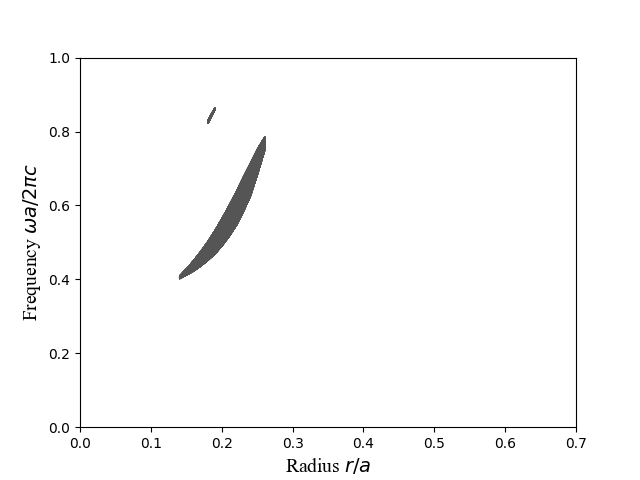
\includegraphics[keepaspectratio, scale=0.45]{results/gap_map/yablonovite_e-10.png}
%     \caption{ヤブロノバイト構造のギャップマップ($\epsilon = 10$)}
%     \label{fig:gapmap_yablonovite_e-10}
%   \end{minipage}
% \end{figure}
% \begin{figure}[h]
%   \begin{minipage}[h]{0.5\linewidth}
%     \centering
%     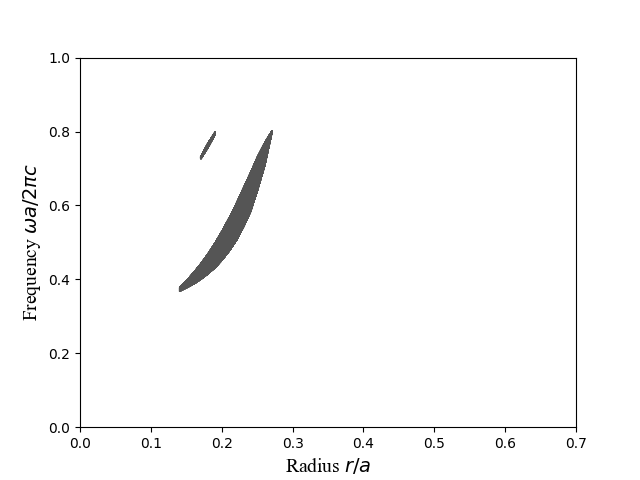
\includegraphics[keepaspectratio, scale=0.45]{results/gap_map/yablonovite_e-13.png}
%     \caption{ヤブロノバイト構造のギャップマップ($\epsilon = 13$)}
%     \label{fig:gapmap_yablonovite_e-13}
%   \end{minipage}
%   \begin{minipage}[h]{0.5\linewidth}
%     \centering
%     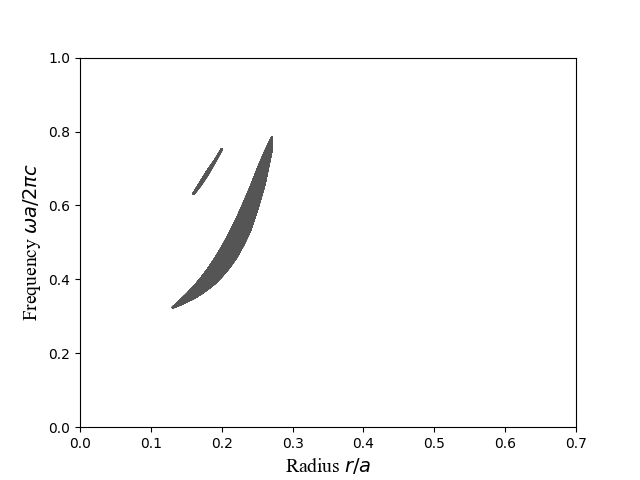
\includegraphics[keepaspectratio, scale=0.45]{results/gap_map/yablonovite_e-15.png}
%     \caption{ヤブロノバイト構造のギャップマップ($\epsilon = 15$)}
%     \label{fig:gapmap_yablonovite_e-15}
%   \end{minipage}
% \end{figure}

% すべての場合についてバンドギャップの存在が確認できた。$\epsilon = 10, 13, 15$の場合にはギャップは2つ存在していた。$\epsilon$が増加するに連れバンドギャップの周波数範囲は増加していることが確認できた。

% 次に各$\epsilon$におけるギャップ-ミッドギャップ比を空気円柱の半径$r / a$を横軸にとってプロットしたグラフを図\ref{fig:yablonovite}に示す。 

% \begin{figure}[htbp]
%   \centering
%   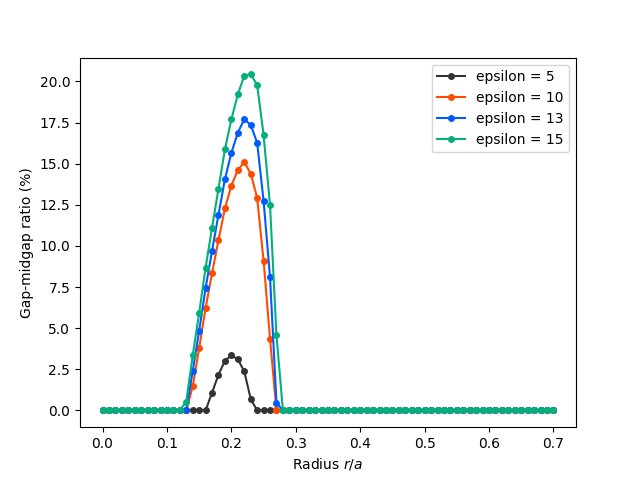
\includegraphics[width=0.8\linewidth]{results/gap_midgap_ratio/yablonovite.png}
%   \caption{ヤブロノバイト構造の空気円柱の半径$r / a$を変化させた際のギャップ-ミッドギャップ比の変化}
%   \label{fig:yablonovite}
% \end{figure}

% $\epsilon = 5$のとき、$r / a = 0.21$でギャップ-ミッドギャップ比は最大となりその値は$3.346 \%$だった。\\
% $\epsilon = 10$のとき、$r / a = 0.23$でギャップ-ミッドギャップ比は最大となりその値は$15.095 \%$だった。\\
% $\epsilon = 13$のとき、$r / a = 0.23$でギャップ-ミッドギャップ比は最大となりその値は$17.692 \%$だった。\\
% $\epsilon = 15$のとき、$r / a = 0.24$でギャップ-ミッドギャップ比は最大となりその値は$20.429 \%$だった。\\



% すべての$\epsilon$においてグラフの形状は非常に似通っており$\epsilon$が大きくなるほどギャップ-ミッドギャップ比の最大値が大きくなっていることが確認できた。\\


% \clearpage

% \subsection{2次元構造の積み重ね}
% 2次元結晶の積み重ねによって作成された3次元結晶内の空気円柱の半径$r / a$を0.01ずつ変化させ、ギャップ-ミッドギャップ比の変化を観察した。この変化を$\epsilon = 5, 10, 12, 15$のそれぞれについて行った。

% 各$\epsilon$におけるギャップマップを以下の図\ref{fig:gapmap_stack_e-5}から図\ref{fig:gapmap_stack_e-15}に示す。
% \begin{figure}[h]
%   \begin{minipage}[h]{0.5\linewidth}
%     \centering
%     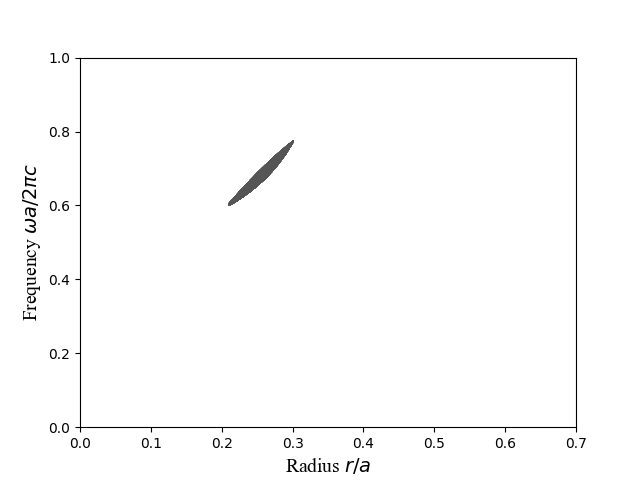
\includegraphics[keepaspectratio, scale=0.45]{results/gap_map/stack_e-5.png}
%     \caption{2次元結晶の積み重ねにより作成された3次元結晶のギャップマップ($\epsilon = 5$)}
%     \label{fig:gapmap_stack_e-5}
%   \end{minipage}
%   \begin{minipage}[h]{0.5\linewidth}
%     \centering
%     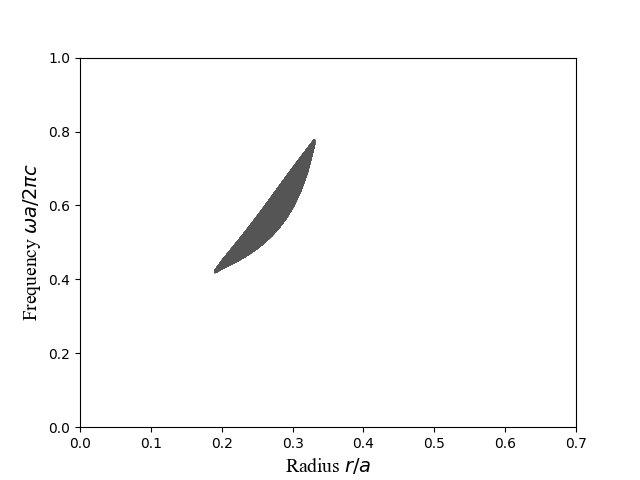
\includegraphics[keepaspectratio, scale=0.45]{results/gap_map/stack_e-10.png}
%     \caption{2次元結晶の積み重ねにより作成された3次元結晶のギャップマップ($\epsilon = 10$)}
%     \label{fig:gapmap_stack_e-10}
%   \end{minipage}
% \end{figure}
% \begin{figure}[h]
%   \begin{minipage}[h]{0.5\linewidth}
%     \centering
%     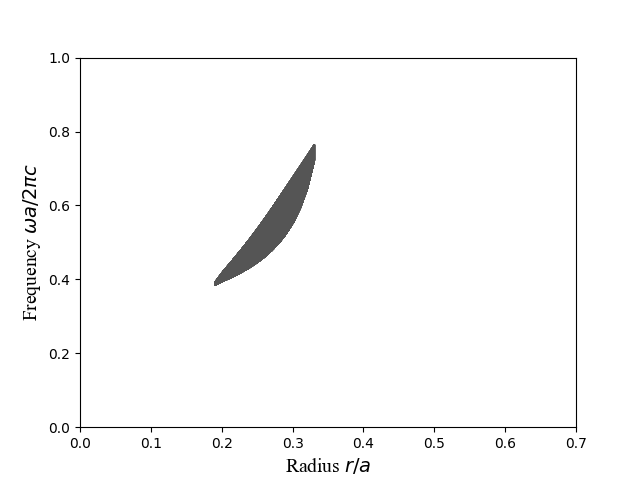
\includegraphics[keepaspectratio, scale=0.45]{results/gap_map/stack_e-12.png}
%     \caption{2次元結晶の積み重ねにより作成された3次元結晶のギャップマップ($\epsilon = 12$)}
%     \label{fig:gapmap_stack_e-13}
%   \end{minipage}
%   \begin{minipage}[h]{0.5\linewidth}
%     \centering
%     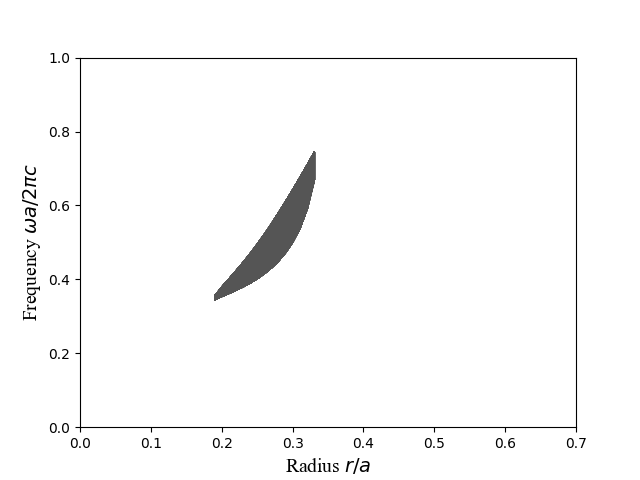
\includegraphics[keepaspectratio, scale=0.45]{results/gap_map/stack_e-15.png}
%     \caption{2次元結晶の積み重ねにより作成された3次元結晶のギャップマップ($\epsilon = 15$)}
%     \label{fig:gapmap_stack_e-15}
%   \end{minipage}
% \end{figure}

% いずれの$\epsilon$についてもバンドギャップの存在が確認できた。$\epsilon$が大きくなるにつれてバンドギャップの周波数範囲は増加していることが確認できた。ギャップの存在している半径$r / a$の範囲は$\epsilon = 5$は他のものに比べ狭いが、他の$\epsilon$については同じであることがわかった。

% 次に各$\epsilon$におけるギャップ-ミッドギャップ比を空気円柱の半径$r / a$を横軸にとってプロットしたグラフを図\ref{fig:stack}に示す。 


% \begin{figure}[htbp]
%   \centering
%   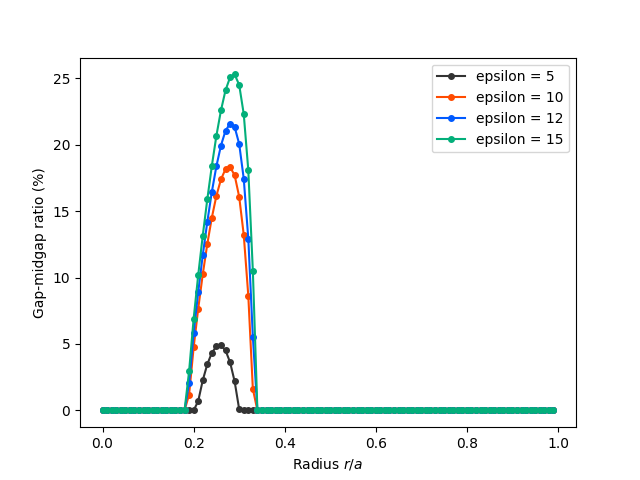
\includegraphics[width=0.8\linewidth]{results/gap_midgap_ratio/stack_crystals.png}
%   \caption{2次元結晶の積み重ねで作成された3次元結晶内の空気円柱の半径$r / a$を変化させた際のギャップ-ミッドギャップ比の変化}
%   \label{fig:stack}
% \end{figure}

% $\epsilon = 5$のとき、$0.22 \leq r / a \leq 0.31$の範囲でギャップは確認でき、$r / a = 0.27$のときギャップ-ミッドギャップ比は最大となり、その値は$4.896 \%$だった。\\
% $\epsilon = 10$のとき、$0.20 \leq r / a \leq 0.34$の範囲でギャップは確認でき、$r / a = 0.29$でギャップ-ミッドギャップ比は最大となり、その値は$18.317 \%$だった。\\
% $\epsilon = 12$のとき、$0.20 \leq r / a \leq 0.34$の範囲でギャップは確認でき、$r / a = 0.29$でギャップ-ミッドギャップ比は最大となり、その値は$21.585 \%$だった。\\
% $\epsilon = 15$のとき、$0.20 \leq r / a \leq 0.34$の範囲でギャップは確認でき、$r / a = 0.30$でギャップ-ミッドギャップ比は最大となり、その値は$25.299 \%$だった。\\



\end{document}